\documentclass[10pt,a4paper,parskip=half]{scrartcl}
\usepackage[utf8]{inputenc}
\usepackage{amsmath}
\usepackage{amsfonts}
\usepackage{amssymb}
\usepackage{mathpazo}
\usepackage{tikz}
\usetikzlibrary{patterns}
\usepackage{stmaryrd} % Für den Widerspruchsblitz :D
\usepackage[left=1cm, right=1cm,
top=1cm, bottom=1cm]{geometry}
\usepackage{fullpage}
\usepackage[german]{babel}
\usepackage{enumerate}
\setlength{\unitlength}{1cm}
\newcommand{\N}{\mathbb{N}}
\newcommand{\A}{\mathcal{A}}
\newcommand{\R}{\mathbb{R}}
\parindent 0mm
\author{Tom}
\title{Analysis 2 - Hausaufgabe 12}

% new commands for vectors
\newcommand{\vectwo}[2]{\begin{pmatrix}#1\\#2\\\end {pmatrix}}
\newcommand{\vecthree}[3]{\begin{pmatrix}#1\\#2\\#3\\\end {pmatrix}}

\usepackage{listings}
\usepackage{courier}
 \lstset{
         basicstyle=\footnotesize\ttfamily, % Standardschrift
         %numbers=left,               % Ort der Zeilennummern
         numberstyle=\tiny,          % Stil der Zeilennummern
         %stepnumber=2,               % Abstand zwischen den Zeilennummern
         numbersep=5pt,              % Abstand der Nummern zum Text
         tabsize=2,                  % Groesse von Tabs
         extendedchars=true,         %
         breaklines=true,            % Zeilen werden Umgebrochen
         keywordstyle=\color{red},
      frame=b,         
 %        keywordstyle=[1]\textbf,    % Stil der Keywords
 %        keywordstyle=[2]\textbf,    %
 %        keywordstyle=[3]\textbf,    %
 %        keywordstyle=[4]\textbf,   \sqrt{\sqrt{}} %
         stringstyle=\color{white}\ttfamily, % Farbe der String
         showspaces=false,            % Leerzeichen anzeigen ?
         showtabs=false,              % Tabs anzeigen ?
         xleftmargin=17pt,
         framexleftmargin=17pt,
         framexrightmargin=5pt,
         framexbottommargin=4pt,
         %backgroundcolor=\color{lightgray},
         showstringspaces=false      % Leerzeichen in Strings anzeigen ?        
 }
 \usepackage{caption}
\DeclareCaptionFont{white}{\color{white}}
\DeclareCaptionFormat{listing}{\colorbox[cmyk]{0.43, 0.35, 0.35,0.01}{\parbox{\textwidth}{\hspace{15pt}#1#2#3}}}
\captionsetup[lstlisting]{format=listing,labelfont=white,textfont=white, singlelinecheck=false, margin=0pt, font={bf,footnotesize}}

\usepackage{color}
\usepackage{enumerate}



\begin{document}
\begin{center}
\textsc{\Large{Analysis 2 - Hausaufgabe 12}} \\
\end{center}
\begin{tabbing}
Tom Nick \hspace{1.4cm}\= 342225\\
Tom Lehmann\> 340621\\
Maximilian Bachl\> 341455
\end{tabbing}
\subsection*{1. Aufgabe}
\begin{enumerate}[(a)]
   \item \ \\
   \begin{minipage}{0.50\columnwidth}
   Ein Vollzylinder mit der Höhe 3 und dem Radius 2.
   \begin{lstlisting}[caption= Mathematica Code für die Menge Z]
   RegionPlot3D[x^2 + y^2 <= 4, {x, -2, 2}, {y, -2, 2}, {z, 0, 3}, 
   AxesLabel -> {x, y, z}]
   \end{lstlisting}
   \end{minipage}
   \begin{minipage}{0.50\columnwidth}
   \begin{center}
   %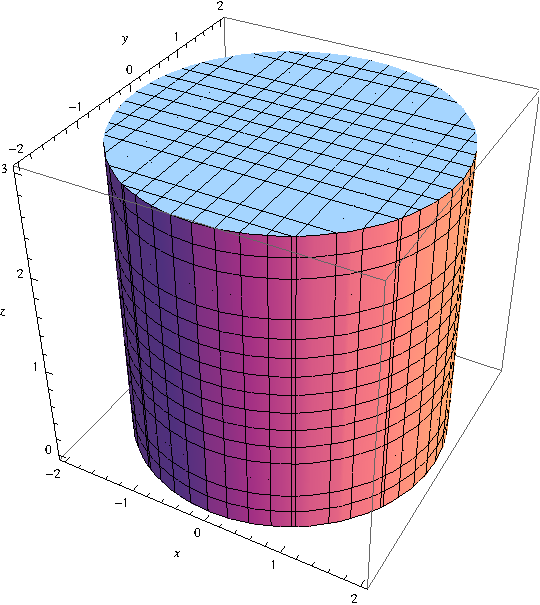
\includegraphics[scale=0.7]{1aZ.pdf} 
   \end{center}
   \end{minipage}
   \ \\
   \begin{minipage}{0.50\columnwidth}
   Ein VollKegel mit der Höhe 1.
   \begin{lstlisting}[caption= Mathematica Code für die Menge K]
   RegionPlot3D[
   RegionPlot3D[
 Sqrt[x^2 + y^2] <= 8 - 2 z, {x, -2, 2}, 
 {y, -2, 2}, {z, 3, 4}, 
 AxesLabel -> {x, y, z}]
   \end{lstlisting}
   \end{minipage}
   \begin{minipage}{0.50\columnwidth}
   \begin{center}
   %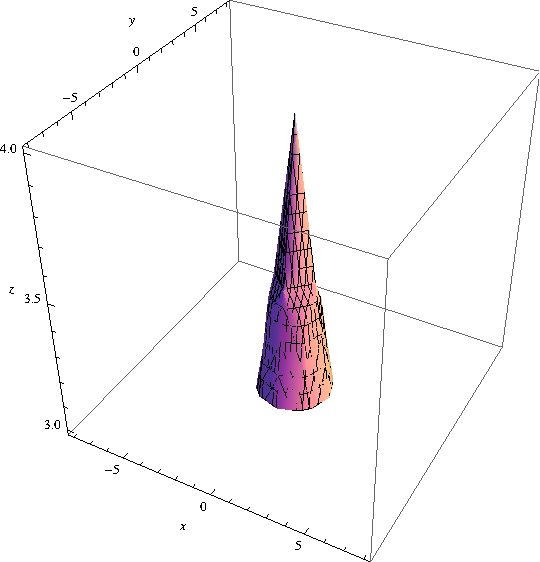
\includegraphics[scale=0.7]{1aK.pdf} 
   \end{center}
   \end{minipage}
   \item  
   Wir benutzen die Zylinderkoordinaten, Funktionaldetermiante ist $r~dr ~ d\varphi ~dz$
   \[ Z = \{ (x,y,z) \in \R^3  \mid x^2 + y^2 \le 4, 0 \le z \le 3\} = \left\{ \vecthree{r \cos \varphi}{r\sin \varphi}{z} \mid r \in [0,2] ,~ \varphi \in [0,2\pi], ~z \in [0,3] \right\} \] 
   Da $Z$ ein kompakter Bereich ist kann der Satz von Gauss angewendet werden:
   \[ \text{div } \vec w(x,y,z) =  yz + x^2 + xy\]
      \begin{align*}
            \iint\limits_{\delta Z} \vec v \cdot d \vec O &= \iiint\limits_{Z} \text{div } \vec w~ r~dr ~d\varphi~ dz \\
            &= \int\limits_{0}^3\int\limits_0^{2\pi}\int\limits_0^2  (rz\sin\varphi + r^2\cos^2\varphi + r\cos\varphi ~r\sin\varphi )r~dr ~d\varphi~ dz \\
            &= \left.\int\limits_{0}^3\int\limits_0^{2\pi}  \frac 13 r^3z \sin \varphi + \frac 14 r^4 \cos^2 \varphi + \frac 14 r^4 \cos \varphi \sin \varphi \right|^2_0  ~d\varphi ~ dz  \\
            &= \int\limits_{0}^3\int\limits_0^{2\pi} \frac 83 z \sin \varphi + 4\cos^2 \varphi + 4\cos \varphi \sin \varphi ~d\varphi ~dz \\
            &= \left.\int\limits_0^3 -\frac 83  z \cos \varphi + 2\varphi + \sin (2\varphi ) - 2\cos^2\varphi \right|^{2\pi}_0 ~dz\\
            &= \int\limits_0^3 - \frac 83 z + 4\pi - 2 + \frac 83z + 2 ~dz \\
            &= \int\limits_0^3  4\pi ~dz \\
            &= 12\pi
      \end{align*}
Wir benutzen die Zylinderkoordinaten, Funktionaldetermiante ist $r~dr ~ d\varphi ~dz$
   \[ K = \{ (x,y,z) \in \R^3  \mid \sqrt{x^2 + y^2} \le 8 - 2z ,~z \in [3,4]\} = \left\{ \vecthree{r \cos \varphi}{r\sin \varphi}{z} \mid 0 \le r \le 8-2z, ~z \in [3,4] ,~ \varphi \in [0,2\pi] \right\} \] 
   Da $K$ ein kompakter Bereich ist kann der Satz von Gauss angewendet werden:
   \[ \text{div } \vec w(x,y,z) =  yz + x^2 + xy\]
      \begin{align*}
            \iint\limits_{\delta K} \vec w \cdot d \vec O &= \iiint\limits_{K} \text{div } \vec w~ r~dr ~d\varphi~ dz \\
            &= \int\limits_{3}^4\int\limits_0^{2\pi}\int\limits_0^{8-2z}  (rz\sin\varphi + r^2\cos^2\varphi + r\cos\varphi ~r\sin\varphi )r~dr ~d\varphi~ dz \\
             &= \left.\int\limits_{3}^4\int\limits_0^{2\pi}  \frac 13 r^3z \sin \varphi + \frac 14 r^4 \cos^2 \varphi + \frac 14 r^4 \cos \varphi \sin \varphi \right|^{8-2z}_0 ~d\varphi~ dz \\
              &= \int\limits_{3}^4\int\limits_0^{2\pi}  \frac 13 (8-2z)^3z\sin \varphi + \frac 14 (8-2z)^4\cos^2\varphi + \frac 14 (8-2z)^4\cos \varphi \sin \varphi  ~d\varphi~ dz \\
               &= \left.\int\limits_{3}^4  - \frac 43 (8-2z)^3z\cos \varphi + (8-2z)^4(\varphi + \sin \varphi \cos \varphi) -(8-2z)^4\cos^2 \varphi  \right|^{2\pi}_{0}~ dz \\
                &= \int\limits_{3}^4 4\pi(z-4)^4   ~ dz \\
                &= \left. \frac 45 \pi (z-4)^5 \right|^4_3    \\
                &= \frac 45 \pi
      \end{align*}
    \item 
    \begin{align*}
        M &= Z \cap K = \left\{ \vecthree{r \cos \varphi}{r\sin \varphi}{3} \mid r \in [0,2] ,~ \varphi \in [0,2\pi] \right\}  \\
        \delta M &=  \left\{ \vecthree{2 \cos \varphi}{2\sin \varphi}{3} \mid ~ \varphi \in [0,2\pi] \right\} 
    \end{align*}
    Nach dem Satz von Stokes gilt:
    \begin{align*}
        \vec v(\vec x) &= \vecthree{6\cos \varphi }{4 \cos \varphi \sin \varphi - 6\sin \varphi}{8 \cos \varphi \sin \varphi - 6\cos \varphi } \\
        \iint\limits_M \text{rot } \vec v \cdot d\vec O  &= \int\limits_{\delta M} \vec v  \cdot \vec ds \\
        &= \int\limits_{0}^{2\pi} \vecthree{6\cos \varphi }{4 \cos \varphi \sin \varphi - 6\sin \varphi}{8 \cos \varphi \sin \varphi - 6\cos \varphi }  \cdot \vecthree{6\cos \varphi }{4 \cos \varphi \sin \varphi - 6\sin \varphi}{8 \cos \varphi \sin \varphi - 6\cos \varphi } ~ d\varphi \\
        &= \int\limits_{0}^{2\pi} 12 \cos^2 \varphi + 6\sin \varphi - 4\sin \varphi \cos \varphi + (6\cos \varphi - 8\sin \varphi)^2 \cos^2 \varphi ~ d \varphi \\
        &= 55 \pi
    \end{align*}
    \item 
    \begin{align*}
      \text{rot } \vec w(x,y,z)  = \left( xz - 0 \right)e_x + \left( xy - yz \right)e_y + \left( 2xy - xz \right)e_z = \vecthree{xz}{xy -yz}{2xy - xz}
    \end{align*}
    \item 

\end{enumerate}


\end{document}

